\documentclass{standalone}
\usepackage{tikz}
\usetikzlibrary{patterns, positioning}


\begin{document}
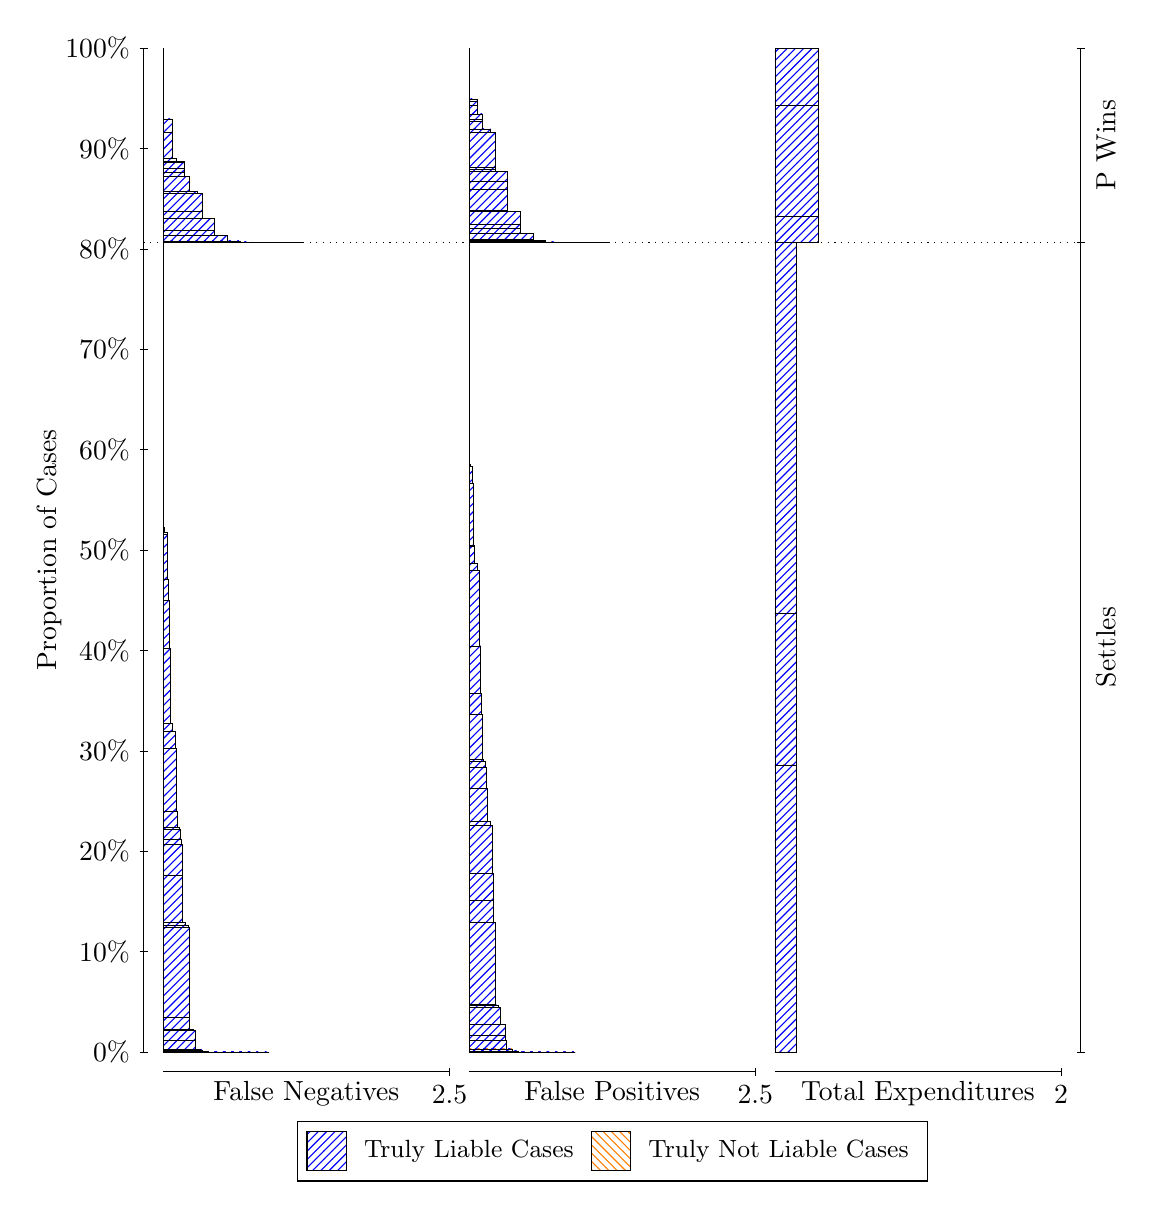
\begin{tikzpicture}
\draw[black, very thin] (1.5,1.75) -- (1.5,14.5);
\node[rotate=90, text=black, anchor=center] at (0.3, 8.125) {Proportion of Cases};
\draw[black, very thin] (1.45,1.75) -- (1.55,1.75);
\node[text=black, anchor=east] at (1.45, 1.75) {0\%};
\draw[black, very thin] (1.45,3.025) -- (1.55,3.025);
\node[text=black, anchor=east] at (1.45, 3.025) {10\%};
\draw[black, very thin] (1.45,4.3) -- (1.55,4.3);
\node[text=black, anchor=east] at (1.45, 4.3) {20\%};
\draw[black, very thin] (1.45,5.575) -- (1.55,5.575);
\node[text=black, anchor=east] at (1.45, 5.575) {30\%};
\draw[black, very thin] (1.45,6.85) -- (1.55,6.85);
\node[text=black, anchor=east] at (1.45, 6.85) {40\%};
\draw[black, very thin] (1.45,8.125) -- (1.55,8.125);
\node[text=black, anchor=east] at (1.45, 8.125) {50\%};
\draw[black, very thin] (1.45,9.4) -- (1.55,9.4);
\node[text=black, anchor=east] at (1.45, 9.4) {60\%};
\draw[black, very thin] (1.45,10.675) -- (1.55,10.675);
\node[text=black, anchor=east] at (1.45, 10.675) {70\%};
\draw[black, very thin] (1.45,11.95) -- (1.55,11.95);
\node[text=black, anchor=east] at (1.45, 11.95) {80\%};
\draw[black, very thin] (1.45,13.225) -- (1.55,13.225);
\node[text=black, anchor=east] at (1.45, 13.225) {90\%};
\draw[black, very thin] (1.45,14.5) -- (1.55,14.5);
\node[text=black, anchor=east] at (1.45, 14.5) {100\%};

\draw[black, very thin] (13.4,1.75) -- (13.4,14.5);
\draw[black, very thin] (13.35,1.75) -- (13.45,1.75);
\node[anchor=west] at (13.35, 1.75) {};
\draw[black, very thin] (13.35,12.035) -- (13.45,12.035);
\node[anchor=west] at (13.35, 12.035) {};
\draw[black, very thin] (13.35,14.5) -- (13.45,14.5);
\node[anchor=west] at (13.35, 14.5) {};

\draw[black, very thin, pattern color=blue, pattern=north east lines] (1.75,1.75) rectangle (3.0943,1.75);
\draw[black, very thin, pattern color=blue, pattern=north east lines] (1.75,1.75) rectangle (2.949,1.75);
\draw[black, very thin, pattern color=blue, pattern=north east lines] (1.75,1.75) rectangle (2.9329,1.75);
\draw[black, very thin, pattern color=blue, pattern=north east lines] (1.75,1.75) rectangle (2.8763,1.75);
\draw[black, very thin, pattern color=blue, pattern=north east lines] (1.75,1.75) rectangle (2.8037,1.75);
\draw[black, very thin, pattern color=blue, pattern=north east lines] (1.75,1.75) rectangle (2.7875,1.75);
\draw[black, very thin, pattern color=blue, pattern=north east lines] (1.75,1.75) rectangle (2.7714,1.75);
\draw[black, very thin, pattern color=blue, pattern=north east lines] (1.75,1.75) rectangle (2.731,1.75);
\draw[black, very thin, pattern color=blue, pattern=north east lines] (1.75,1.75) rectangle (2.7149,1.75);
\draw[black, very thin, pattern color=blue, pattern=north east lines] (1.75,1.75) rectangle (2.6583,1.75);
\draw[black, very thin, pattern color=blue, pattern=north east lines] (1.75,1.75) rectangle (2.6422,1.75);
\draw[black, very thin, pattern color=blue, pattern=north east lines] (1.75,1.75) rectangle (2.626,1.75);
\draw[black, very thin, pattern color=blue, pattern=north east lines] (1.75,1.75) rectangle (2.6099,1.75);
\draw[black, very thin, pattern color=blue, pattern=north east lines] (1.75,1.75) rectangle (2.5857,1.75);
\draw[black, very thin, pattern color=blue, pattern=north east lines] (1.75,1.75) rectangle (2.5695,1.75);
\draw[black, very thin, pattern color=blue, pattern=north east lines] (1.75,1.75) rectangle (2.5534,1.75);
\draw[black, very thin, pattern color=blue, pattern=north east lines] (1.75,1.75) rectangle (2.513,1.75);
\draw[black, very thin, pattern color=blue, pattern=north east lines] (1.75,1.75) rectangle (2.4969,1.75);
\draw[black, very thin, pattern color=blue, pattern=north east lines] (1.75,1.75) rectangle (2.4807,1.7501);
\draw[black, very thin, pattern color=blue, pattern=north east lines] (1.75,1.7501) rectangle (2.4646,1.7501);
\draw[black, very thin, pattern color=blue, pattern=north east lines] (1.75,1.7501) rectangle (2.4484,1.7501);
\draw[black, very thin, pattern color=blue, pattern=north east lines] (1.75,1.7501) rectangle (2.4403,1.7501);
\draw[black, very thin, pattern color=blue, pattern=north east lines] (1.75,1.7501) rectangle (2.4242,1.7501);
\draw[black, very thin, pattern color=blue, pattern=north east lines] (1.75,1.7501) rectangle (2.408,1.7505);
\draw[black, very thin, pattern color=blue, pattern=north east lines] (1.75,1.7505) rectangle (2.3919,1.7505);
\draw[black, very thin, pattern color=blue, pattern=north east lines] (1.75,1.7505) rectangle (2.3515,1.7506);
\draw[black, very thin, pattern color=blue, pattern=north east lines] (1.75,1.7506) rectangle (2.3354,1.7506);
\draw[black, very thin, pattern color=blue, pattern=north east lines] (1.75,1.7506) rectangle (2.3192,1.7563);
\draw[black, very thin, pattern color=blue, pattern=north east lines] (1.75,1.7563) rectangle (2.3031,1.7563);
\draw[black, very thin, pattern color=blue, pattern=north east lines] (1.75,1.7563) rectangle (2.2869,1.7564);
\draw[black, very thin, pattern color=blue, pattern=north east lines] (1.75,1.7564) rectangle (2.2789,1.7567);
\draw[black, very thin, pattern color=blue, pattern=north east lines] (1.75,1.7567) rectangle (2.2627,1.7567);
\draw[black, very thin, pattern color=blue, pattern=north east lines] (1.75,1.7567) rectangle (2.2466,1.7773);
\draw[black, very thin, pattern color=blue, pattern=north east lines] (1.75,1.7773) rectangle (2.2304,1.7774);
\draw[black, very thin, pattern color=blue, pattern=north east lines] (1.75,1.7774) rectangle (2.2223,1.7785);
\draw[black, very thin, pattern color=blue, pattern=north east lines] (1.75,1.7785) rectangle (2.19,1.7804);
\draw[black, very thin, pattern color=blue, pattern=north east lines] (1.75,1.7804) rectangle (2.1739,1.7804);
\draw[black, very thin, pattern color=blue, pattern=north east lines] (1.75,1.7804) rectangle (2.1577,1.9016);
\draw[black, very thin, pattern color=blue, pattern=north east lines] (1.75,1.9016) rectangle (2.1497,2.0237);
\draw[black, very thin, pattern color=blue, pattern=north east lines] (1.75,2.0237) rectangle (2.1416,2.0291);
\draw[black, very thin, pattern color=blue, pattern=north east lines] (1.75,2.0291) rectangle (2.1254,2.0348);
\draw[black, very thin, pattern color=blue, pattern=north east lines] (1.75,2.0348) rectangle (2.1174,2.0402);
\draw[black, very thin, pattern color=blue, pattern=north east lines] (1.75,2.0402) rectangle (2.1012,2.0403);
\draw[black, very thin, pattern color=blue, pattern=north east lines] (1.75,2.0403) rectangle (2.0851,2.1908);
\draw[black, very thin, pattern color=blue, pattern=north east lines] (1.75,2.1908) rectangle (2.077,3.3323);
\draw[black, very thin, pattern color=blue, pattern=north east lines] (1.75,3.3323) rectangle (2.0689,3.3342);
\draw[black, very thin, pattern color=blue, pattern=north east lines] (1.75,3.3342) rectangle (2.0609,3.3615);
\draw[black, very thin, pattern color=blue, pattern=north east lines] (1.75,3.3615) rectangle (2.0286,3.3942);
\draw[black, very thin, pattern color=blue, pattern=north east lines] (1.75,3.3942) rectangle (2.0124,3.3942);
\draw[black, very thin, pattern color=blue, pattern=north east lines] (1.75,3.3942) rectangle (1.9963,3.9929);
\draw[black, very thin, pattern color=blue, pattern=north east lines] (1.75,3.9929) rectangle (1.9882,4.384);
\draw[black, very thin, pattern color=blue, pattern=north east lines] (1.75,4.384) rectangle (1.9801,4.4576);
\draw[black, very thin, pattern color=blue, pattern=north east lines] (1.75,4.4576) rectangle (1.964,4.5756);
\draw[black, very thin, pattern color=blue, pattern=north east lines] (1.75,4.5756) rectangle (1.9559,4.6019);
\draw[black, very thin, pattern color=blue, pattern=north east lines] (1.75,4.6019) rectangle (1.9397,4.6019);
\draw[black, very thin, pattern color=blue, pattern=north east lines] (1.75,4.6019) rectangle (1.9236,4.8131);
\draw[black, very thin, pattern color=blue, pattern=north east lines] (1.75,4.8131) rectangle (1.9155,5.6055);
\draw[black, very thin, pattern color=blue, pattern=north east lines] (1.75,5.6055) rectangle (1.9074,5.6106);
\draw[black, very thin, pattern color=blue, pattern=north east lines] (1.75,5.6106) rectangle (1.8994,5.8244);
\draw[black, very thin, pattern color=blue, pattern=north east lines] (1.75,5.8244) rectangle (1.8671,5.9195);
\draw[black, very thin, pattern color=blue, pattern=north east lines] (1.75,5.9195) rectangle (1.8509,5.9199);
\draw[black, very thin, pattern color=blue, pattern=north east lines] (1.75,5.9199) rectangle (1.8348,6.8774);
\draw[black, very thin, pattern color=blue, pattern=north east lines] (1.75,6.8774) rectangle (1.8267,7.4837);
\draw[black, very thin, pattern color=blue, pattern=north east lines] (1.75,7.4837) rectangle (1.8186,7.7511);
\draw[black, very thin, pattern color=blue, pattern=north east lines] (1.75,7.7511) rectangle (1.8025,8.3224);
\draw[black, very thin, pattern color=blue, pattern=north east lines] (1.75,8.3224) rectangle (1.7944,8.3486);
\draw[black, very thin, pattern color=blue, pattern=north east lines] (1.75,8.3486) rectangle (1.7783,8.3487);
\draw[black, very thin, pattern color=blue, pattern=north east lines] (1.75,8.3487) rectangle (1.7621,8.4157);
\draw[black, very thin, pattern color=blue, pattern=north east lines] (1.75,8.4157) rectangle (1.754,8.6831);
\draw[black, very thin, pattern color=orange, pattern=north west lines] (1.75,8.6831) rectangle (1.75,8.6831);
\draw[black, very thin, pattern color=blue, pattern=north east lines] (1.75,8.6831) rectangle (1.75,12.035);
\draw[black, very thin, pattern color=blue, pattern=north east lines] (1.75,12.035) rectangle (3.5303,12.035);
\draw[black, very thin, pattern color=blue, pattern=north east lines] (1.75,12.035) rectangle (3.3689,12.035);
\draw[black, very thin, pattern color=blue, pattern=north east lines] (1.75,12.035) rectangle (3.2074,12.035);
\draw[black, very thin, pattern color=blue, pattern=north east lines] (1.75,12.035) rectangle (3.0459,12.035);
\draw[black, very thin, pattern color=blue, pattern=north east lines] (1.75,12.035) rectangle (2.9894,12.035);
\draw[black, very thin, pattern color=blue, pattern=north east lines] (1.75,12.035) rectangle (2.8844,12.036);
\draw[black, very thin, pattern color=blue, pattern=north east lines] (1.75,12.036) rectangle (2.8844,12.037);
\draw[black, very thin, pattern color=blue, pattern=north east lines] (1.75,12.037) rectangle (2.8279,12.037);
\draw[black, very thin, pattern color=blue, pattern=north east lines] (1.75,12.037) rectangle (2.7229,12.044);
\draw[black, very thin, pattern color=blue, pattern=north east lines] (1.75,12.044) rectangle (2.7229,12.051);
\draw[black, very thin, pattern color=blue, pattern=north east lines] (1.75,12.051) rectangle (2.6664,12.051);
\draw[black, very thin, pattern color=blue, pattern=north east lines] (1.75,12.051) rectangle (2.5614,12.117);
\draw[black, very thin, pattern color=blue, pattern=north east lines] (1.75,12.117) rectangle (2.5614,12.12);
\draw[black, very thin, pattern color=blue, pattern=north east lines] (1.75,12.12) rectangle (2.5049,12.12);
\draw[black, very thin, pattern color=blue, pattern=north east lines] (1.75,12.12) rectangle (2.5049,12.12);
\draw[black, very thin, pattern color=blue, pattern=north east lines] (1.75,12.12) rectangle (2.4,12.188);
\draw[black, very thin, pattern color=blue, pattern=north east lines] (1.75,12.188) rectangle (2.4,12.332);
\draw[black, very thin, pattern color=blue, pattern=north east lines] (1.75,12.332) rectangle (2.3434,12.332);
\draw[black, very thin, pattern color=blue, pattern=north east lines] (1.75,12.332) rectangle (2.3434,12.332);
\draw[black, very thin, pattern color=blue, pattern=north east lines] (1.75,12.332) rectangle (2.3434,12.333);
\draw[black, very thin, pattern color=blue, pattern=north east lines] (1.75,12.333) rectangle (2.2385,12.425);
\draw[black, very thin, pattern color=blue, pattern=north east lines] (1.75,12.425) rectangle (2.2385,12.651);
\draw[black, very thin, pattern color=blue, pattern=north east lines] (1.75,12.651) rectangle (2.2385,12.658);
\draw[black, very thin, pattern color=blue, pattern=north east lines] (1.75,12.658) rectangle (2.182,12.658);
\draw[black, very thin, pattern color=blue, pattern=north east lines] (1.75,12.658) rectangle (2.182,12.677);
\draw[black, very thin, pattern color=blue, pattern=north east lines] (1.75,12.677) rectangle (2.182,12.68);
\draw[black, very thin, pattern color=blue, pattern=north east lines] (1.75,12.68) rectangle (2.077,12.87);
\draw[black, very thin, pattern color=blue, pattern=north east lines] (1.75,12.87) rectangle (2.0205,12.928);
\draw[black, very thin, pattern color=blue, pattern=north east lines] (1.75,12.928) rectangle (2.0205,12.969);
\draw[black, very thin, pattern color=blue, pattern=north east lines] (1.75,12.969) rectangle (2.0205,13.047);
\draw[black, very thin, pattern color=blue, pattern=north east lines] (1.75,13.047) rectangle (2.0205,13.063);
\draw[black, very thin, pattern color=blue, pattern=north east lines] (1.75,13.063) rectangle (1.9155,13.063);
\draw[black, very thin, pattern color=blue, pattern=north east lines] (1.75,13.063) rectangle (1.9155,13.103);
\draw[black, very thin, pattern color=blue, pattern=north east lines] (1.75,13.103) rectangle (1.9155,13.103);
\draw[black, very thin, pattern color=blue, pattern=north east lines] (1.75,13.103) rectangle (1.859,13.43);
\draw[black, very thin, pattern color=blue, pattern=north east lines] (1.75,13.43) rectangle (1.859,13.6);
\draw[black, very thin, pattern color=blue, pattern=north east lines] (1.75,13.6) rectangle (1.754,13.6);
\draw[black, very thin, pattern color=blue, pattern=north east lines] (1.75,13.6) rectangle (1.754,13.6);
\draw[black, very thin, pattern color=orange, pattern=north west lines] (1.75,13.6) rectangle (1.75,13.6);
\draw[black, very thin, pattern color=blue, pattern=north east lines] (1.75,13.6) rectangle (1.75,14.5);
\draw[black, very thin, pattern color=orange, pattern=north west lines] (5.6333,1.75) rectangle (6.9777,1.75);
\draw[black, very thin, pattern color=blue, pattern=north east lines] (5.6333,1.75) rectangle (6.9777,1.75);
\draw[black, very thin, pattern color=orange, pattern=north west lines] (5.6333,1.75) rectangle (6.905,1.75);
\draw[black, very thin, pattern color=blue, pattern=north east lines] (5.6333,1.75) rectangle (6.905,1.75);
\draw[black, very thin, pattern color=orange, pattern=north west lines] (5.6333,1.75) rectangle (6.8323,1.75);
\draw[black, very thin, pattern color=blue, pattern=north east lines] (5.6333,1.75) rectangle (6.8323,1.75);
\draw[black, very thin, pattern color=blue, pattern=north east lines] (5.6333,1.75) rectangle (6.8162,1.75);
\draw[black, very thin, pattern color=blue, pattern=north east lines] (5.6333,1.75) rectangle (6.7435,1.75);
\draw[black, very thin, pattern color=blue, pattern=north east lines] (5.6333,1.75) rectangle (6.6709,1.75);
\draw[black, very thin, pattern color=blue, pattern=north east lines] (5.6333,1.75) rectangle (6.6547,1.75);
\draw[black, very thin, pattern color=orange, pattern=north west lines] (5.6333,1.75) rectangle (6.6143,1.75);
\draw[black, very thin, pattern color=blue, pattern=north east lines] (5.6333,1.75) rectangle (6.6143,1.75);
\draw[black, very thin, pattern color=blue, pattern=north east lines] (5.6333,1.75) rectangle (6.582,1.75);
\draw[black, very thin, pattern color=orange, pattern=north west lines] (5.6333,1.75) rectangle (6.5417,1.75);
\draw[black, very thin, pattern color=blue, pattern=north east lines] (5.6333,1.75) rectangle (6.5417,1.75);
\draw[black, very thin, pattern color=blue, pattern=north east lines] (5.6333,1.75) rectangle (6.5094,1.75);
\draw[black, very thin, pattern color=blue, pattern=north east lines] (5.6333,1.75) rectangle (6.4932,1.75);
\draw[black, very thin, pattern color=orange, pattern=north west lines] (5.6333,1.75) rectangle (6.469,1.75);
\draw[black, very thin, pattern color=blue, pattern=north east lines] (5.6333,1.75) rectangle (6.469,1.75);
\draw[black, very thin, pattern color=blue, pattern=north east lines] (5.6333,1.75) rectangle (6.4529,1.75);
\draw[black, very thin, pattern color=blue, pattern=north east lines] (5.6333,1.75) rectangle (6.4206,1.75);
\draw[black, very thin, pattern color=orange, pattern=north west lines] (5.6333,1.75) rectangle (6.3963,1.75);
\draw[black, very thin, pattern color=blue, pattern=north east lines] (5.6333,1.75) rectangle (6.3963,1.75);
\draw[black, very thin, pattern color=blue, pattern=north east lines] (5.6333,1.75) rectangle (6.3802,1.75);
\draw[black, very thin, pattern color=blue, pattern=north east lines] (5.6333,1.75) rectangle (6.3479,1.7505);
\draw[black, very thin, pattern color=blue, pattern=north east lines] (5.6333,1.7505) rectangle (6.3317,1.7505);
\draw[black, very thin, pattern color=orange, pattern=north west lines] (5.6333,1.7505) rectangle (6.3237,1.7505);
\draw[black, very thin, pattern color=blue, pattern=north east lines] (5.6333,1.7505) rectangle (6.3237,1.7505);
\draw[black, very thin, pattern color=blue, pattern=north east lines] (5.6333,1.7505) rectangle (6.3075,1.7505);
\draw[black, very thin, pattern color=blue, pattern=north east lines] (5.6333,1.7505) rectangle (6.2914,1.7505);
\draw[black, very thin, pattern color=blue, pattern=north east lines] (5.6333,1.7505) rectangle (6.2591,1.753);
\draw[black, very thin, pattern color=orange, pattern=north west lines] (5.6333,1.753) rectangle (6.251,1.753);
\draw[black, very thin, pattern color=blue, pattern=north east lines] (5.6333,1.753) rectangle (6.251,1.7649);
\draw[black, very thin, pattern color=blue, pattern=north east lines] (5.6333,1.7649) rectangle (6.2349,1.7649);
\draw[black, very thin, pattern color=blue, pattern=north east lines] (5.6333,1.7649) rectangle (6.2187,1.7651);
\draw[black, very thin, pattern color=blue, pattern=north east lines] (5.6333,1.7651) rectangle (6.1864,1.7889);
\draw[black, very thin, pattern color=orange, pattern=north west lines] (5.6333,1.7889) rectangle (6.1783,1.7889);
\draw[black, very thin, pattern color=blue, pattern=north east lines] (5.6333,1.7889) rectangle (6.1783,1.7889);
\draw[black, very thin, pattern color=blue, pattern=north east lines] (5.6333,1.7889) rectangle (6.1703,1.7894);
\draw[black, very thin, pattern color=blue, pattern=north east lines] (5.6333,1.7894) rectangle (6.1622,1.7895);
\draw[black, very thin, pattern color=blue, pattern=north east lines] (5.6333,1.7895) rectangle (6.146,1.7895);
\draw[black, very thin, pattern color=blue, pattern=north east lines] (5.6333,1.7895) rectangle (6.1299,1.7898);
\draw[black, very thin, pattern color=orange, pattern=north west lines] (5.6333,1.7898) rectangle (6.1057,1.7898);
\draw[black, very thin, pattern color=blue, pattern=north east lines] (5.6333,1.7898) rectangle (6.1057,1.9011);
\draw[black, very thin, pattern color=blue, pattern=north east lines] (5.6333,1.9011) rectangle (6.0976,1.9594);
\draw[black, very thin, pattern color=blue, pattern=north east lines] (5.6333,1.9594) rectangle (6.0895,2.0986);
\draw[black, very thin, pattern color=blue, pattern=north east lines] (5.6333,2.0986) rectangle (6.0734,2.0987);
\draw[black, very thin, pattern color=blue, pattern=north east lines] (5.6333,2.0987) rectangle (6.0572,2.1053);
\draw[black, very thin, pattern color=blue, pattern=north east lines] (5.6333,2.1053) rectangle (6.0249,2.3165);
\draw[black, very thin, pattern color=blue, pattern=north east lines] (5.6333,2.3165) rectangle (6.0169,2.3167);
\draw[black, very thin, pattern color=blue, pattern=north east lines] (5.6333,2.3167) rectangle (6.0088,2.3429);
\draw[black, very thin, pattern color=blue, pattern=north east lines] (5.6333,2.3429) rectangle (6.0007,2.3482);
\draw[black, very thin, pattern color=blue, pattern=north east lines] (5.6333,2.3482) rectangle (5.9846,2.3482);
\draw[black, very thin, pattern color=blue, pattern=north east lines] (5.6333,2.3482) rectangle (5.9684,2.3536);
\draw[black, very thin, pattern color=orange, pattern=north west lines] (5.6333,2.3536) rectangle (5.9603,2.3536);
\draw[black, very thin, pattern color=blue, pattern=north east lines] (5.6333,2.3536) rectangle (5.9603,3.3942);
\draw[black, very thin, pattern color=blue, pattern=north east lines] (5.6333,3.3942) rectangle (5.9442,3.6761);
\draw[black, very thin, pattern color=blue, pattern=north east lines] (5.6333,3.6761) rectangle (5.9361,4.0168);
\draw[black, very thin, pattern color=blue, pattern=north east lines] (5.6333,4.0168) rectangle (5.928,4.6231);
\draw[black, very thin, pattern color=blue, pattern=north east lines] (5.6333,4.6231) rectangle (5.9119,4.6236);
\draw[black, very thin, pattern color=blue, pattern=north east lines] (5.6333,4.6236) rectangle (5.8957,4.6765);
\draw[black, very thin, pattern color=blue, pattern=north east lines] (5.6333,4.6765) rectangle (5.8634,5.0997);
\draw[black, very thin, pattern color=blue, pattern=north east lines] (5.6333,5.0997) rectangle (5.8554,5.102);
\draw[black, very thin, pattern color=blue, pattern=north east lines] (5.6333,5.102) rectangle (5.8473,5.3695);
\draw[black, very thin, pattern color=blue, pattern=north east lines] (5.6333,5.3695) rectangle (5.8392,5.4365);
\draw[black, very thin, pattern color=blue, pattern=north east lines] (5.6333,5.4365) rectangle (5.8231,5.4365);
\draw[black, very thin, pattern color=blue, pattern=north east lines] (5.6333,5.4365) rectangle (5.8069,5.4628);
\draw[black, very thin, pattern color=blue, pattern=north east lines] (5.6333,5.4628) rectangle (5.7989,6.034);
\draw[black, very thin, pattern color=blue, pattern=north east lines] (5.6333,6.034) rectangle (5.7827,6.3015);
\draw[black, very thin, pattern color=blue, pattern=north east lines] (5.6333,6.3015) rectangle (5.7746,6.9077);
\draw[black, very thin, pattern color=blue, pattern=north east lines] (5.6333,6.9077) rectangle (5.7666,7.8652);
\draw[black, very thin, pattern color=blue, pattern=north east lines] (5.6333,7.8652) rectangle (5.7504,7.8657);
\draw[black, very thin, pattern color=blue, pattern=north east lines] (5.6333,7.8657) rectangle (5.7343,7.9607);
\draw[black, very thin, pattern color=blue, pattern=north east lines] (5.6333,7.9607) rectangle (5.702,8.1746);
\draw[black, very thin, pattern color=blue, pattern=north east lines] (5.6333,8.1746) rectangle (5.6939,8.1797);
\draw[black, very thin, pattern color=blue, pattern=north east lines] (5.6333,8.1797) rectangle (5.6858,8.9721);
\draw[black, very thin, pattern color=blue, pattern=north east lines] (5.6333,8.9721) rectangle (5.6777,9.1833);
\draw[black, very thin, pattern color=blue, pattern=north east lines] (5.6333,9.1833) rectangle (5.6616,9.1833);
\draw[black, very thin, pattern color=blue, pattern=north east lines] (5.6333,9.1833) rectangle (5.6454,9.2096);
\draw[black, very thin, pattern color=blue, pattern=north east lines] (5.6333,9.2096) rectangle (5.6374,9.3276);
\draw[black, very thin, pattern color=blue, pattern=north east lines] (5.6333,9.3276) rectangle (5.6333,12.035);
\draw[black, very thin, pattern color=orange, pattern=north west lines] (5.6333,12.035) rectangle (7.4137,12.035);
\draw[black, very thin, pattern color=blue, pattern=north east lines] (5.6333,12.035) rectangle (7.4137,12.035);
\draw[black, very thin, pattern color=orange, pattern=north west lines] (5.6333,12.035) rectangle (7.2522,12.035);
\draw[black, very thin, pattern color=blue, pattern=north east lines] (5.6333,12.035) rectangle (7.2522,12.035);
\draw[black, very thin, pattern color=orange, pattern=north west lines] (5.6333,12.035) rectangle (7.0907,12.035);
\draw[black, very thin, pattern color=blue, pattern=north east lines] (5.6333,12.035) rectangle (7.0907,12.035);
\draw[black, very thin, pattern color=blue, pattern=north east lines] (5.6333,12.035) rectangle (6.9292,12.035);
\draw[black, very thin, pattern color=blue, pattern=north east lines] (5.6333,12.035) rectangle (6.9292,12.035);
\draw[black, very thin, pattern color=orange, pattern=north west lines] (5.6333,12.035) rectangle (6.9292,12.035);
\draw[black, very thin, pattern color=blue, pattern=north east lines] (5.6333,12.035) rectangle (6.9292,12.035);
\draw[black, very thin, pattern color=blue, pattern=north east lines] (5.6333,12.035) rectangle (6.7677,12.036);
\draw[black, very thin, pattern color=orange, pattern=north west lines] (5.6333,12.036) rectangle (6.7677,12.036);
\draw[black, very thin, pattern color=blue, pattern=north east lines] (5.6333,12.036) rectangle (6.7677,12.036);
\draw[black, very thin, pattern color=blue, pattern=north east lines] (5.6333,12.036) rectangle (6.7677,12.037);
\draw[black, very thin, pattern color=orange, pattern=north west lines] (5.6333,12.037) rectangle (6.7112,12.037);
\draw[black, very thin, pattern color=blue, pattern=north east lines] (5.6333,12.037) rectangle (6.7112,12.037);
\draw[black, very thin, pattern color=blue, pattern=north east lines] (5.6333,12.037) rectangle (6.6063,12.049);
\draw[black, very thin, pattern color=orange, pattern=north west lines] (5.6333,12.049) rectangle (6.6063,12.049);
\draw[black, very thin, pattern color=blue, pattern=north east lines] (5.6333,12.049) rectangle (6.6063,12.053);
\draw[black, very thin, pattern color=orange, pattern=north west lines] (5.6333,12.053) rectangle (6.5497,12.053);
\draw[black, very thin, pattern color=blue, pattern=north east lines] (5.6333,12.053) rectangle (6.5497,12.053);
\draw[black, very thin, pattern color=blue, pattern=north east lines] (5.6333,12.053) rectangle (6.4448,12.069);
\draw[black, very thin, pattern color=orange, pattern=north west lines] (5.6333,12.069) rectangle (6.4448,12.069);
\draw[black, very thin, pattern color=blue, pattern=north east lines] (5.6333,12.069) rectangle (6.4448,12.143);
\draw[black, very thin, pattern color=orange, pattern=north west lines] (5.6333,12.143) rectangle (6.3883,12.143);
\draw[black, very thin, pattern color=blue, pattern=north east lines] (5.6333,12.143) rectangle (6.3883,12.143);
\draw[black, very thin, pattern color=blue, pattern=north east lines] (5.6333,12.143) rectangle (6.2833,12.208);
\draw[black, very thin, pattern color=blue, pattern=north east lines] (5.6333,12.208) rectangle (6.2833,12.263);
\draw[black, very thin, pattern color=orange, pattern=north west lines] (5.6333,12.263) rectangle (6.2833,12.263);
\draw[black, very thin, pattern color=blue, pattern=north east lines] (5.6333,12.263) rectangle (6.2833,12.424);
\draw[black, very thin, pattern color=orange, pattern=north west lines] (5.6333,12.424) rectangle (6.2268,12.424);
\draw[black, very thin, pattern color=blue, pattern=north east lines] (5.6333,12.424) rectangle (6.2268,12.424);
\draw[black, very thin, pattern color=blue, pattern=north east lines] (5.6333,12.424) rectangle (6.2268,12.424);
\draw[black, very thin, pattern color=blue, pattern=north east lines] (5.6333,12.424) rectangle (6.1218,12.44);
\draw[black, very thin, pattern color=blue, pattern=north east lines] (5.6333,12.44) rectangle (6.1218,12.703);
\draw[black, very thin, pattern color=blue, pattern=north east lines] (5.6333,12.703) rectangle (6.1218,12.807);
\draw[black, very thin, pattern color=blue, pattern=north east lines] (5.6333,12.807) rectangle (6.1218,12.935);
\draw[black, very thin, pattern color=orange, pattern=north west lines] (5.6333,12.935) rectangle (6.0653,12.935);
\draw[black, very thin, pattern color=blue, pattern=north east lines] (5.6333,12.935) rectangle (6.0653,12.935);
\draw[black, very thin, pattern color=blue, pattern=north east lines] (5.6333,12.935) rectangle (6.0653,12.935);
\draw[black, very thin, pattern color=blue, pattern=north east lines] (5.6333,12.935) rectangle (5.9603,12.959);
\draw[black, very thin, pattern color=blue, pattern=north east lines] (5.6333,12.959) rectangle (5.9603,12.98);
\draw[black, very thin, pattern color=blue, pattern=north east lines] (5.6333,12.98) rectangle (5.9603,13.432);
\draw[black, very thin, pattern color=orange, pattern=north west lines] (5.6333,13.432) rectangle (5.9038,13.432);
\draw[black, very thin, pattern color=blue, pattern=north east lines] (5.6333,13.432) rectangle (5.9038,13.471);
\draw[black, very thin, pattern color=blue, pattern=north east lines] (5.6333,13.471) rectangle (5.9038,13.472);
\draw[black, very thin, pattern color=blue, pattern=north east lines] (5.6333,13.472) rectangle (5.9038,13.472);
\draw[black, very thin, pattern color=blue, pattern=north east lines] (5.6333,13.472) rectangle (5.7989,13.572);
\draw[black, very thin, pattern color=blue, pattern=north east lines] (5.6333,13.572) rectangle (5.7989,13.589);
\draw[black, very thin, pattern color=blue, pattern=north east lines] (5.6333,13.589) rectangle (5.7989,13.665);
\draw[black, very thin, pattern color=blue, pattern=north east lines] (5.6333,13.665) rectangle (5.7423,13.775);
\draw[black, very thin, pattern color=orange, pattern=north west lines] (5.6333,13.775) rectangle (5.7423,13.775);
\draw[black, very thin, pattern color=blue, pattern=north east lines] (5.6333,13.775) rectangle (5.7423,13.821);
\draw[black, very thin, pattern color=blue, pattern=north east lines] (5.6333,13.821) rectangle (5.7423,13.855);
\draw[black, very thin, pattern color=blue, pattern=north east lines] (5.6333,13.855) rectangle (5.6374,13.877);
\draw[black, very thin, pattern color=blue, pattern=north east lines] (5.6333,13.877) rectangle (5.6333,14.5);
\draw[black, very thin, pattern color=orange, pattern=north west lines] (9.5167,1.75) rectangle (9.7892,1.75);
\draw[black, very thin, pattern color=blue, pattern=north east lines] (9.5167,1.75) rectangle (9.7892,5.3962);
\draw[black, very thin, pattern color=orange, pattern=north west lines] (9.5167,5.3962) rectangle (9.7892,5.3962);
\draw[black, very thin, pattern color=blue, pattern=north east lines] (9.5167,5.3962) rectangle (9.7892,7.3212);
\draw[black, very thin, pattern color=orange, pattern=north west lines] (9.5167,7.3212) rectangle (9.7892,7.3212);
\draw[black, very thin, pattern color=blue, pattern=north east lines] (9.5167,7.3212) rectangle (9.7892,12.035);
\draw[black, very thin, pattern color=orange, pattern=north west lines] (9.5167,12.035) rectangle (10.062,12.035);
\draw[black, very thin, pattern color=blue, pattern=north east lines] (9.5167,12.035) rectangle (10.062,12.358);
\draw[black, very thin, pattern color=orange, pattern=north west lines] (9.5167,12.358) rectangle (10.062,12.358);
\draw[black, very thin, pattern color=blue, pattern=north east lines] (9.5167,12.358) rectangle (10.062,13.768);
\draw[black, very thin, pattern color=orange, pattern=north west lines] (9.5167,13.768) rectangle (10.062,13.768);
\draw[black, very thin, pattern color=blue, pattern=north east lines] (9.5167,13.768) rectangle (10.062,14.5);
\draw[black, dotted] (1.5,12.035) -- (13.4,12.035);
\draw[black, very thin] (1.75,1.5) -- (5.3833,1.5);
\node[text=black, anchor=north] at (3.5667, 1.5) {False Negatives};
\draw[black, very thin] (5.3833,1.45) -- (5.3833,1.55);
\node[text=black, anchor=north] at (5.3833, 1.45) {2.5};

\draw[black, very thin] (5.6333,1.5) -- (9.2667,1.5);
\node[text=black, anchor=north] at (7.45, 1.5) {False Positives};
\draw[black, very thin] (9.2667,1.45) -- (9.2667,1.55);
\node[text=black, anchor=north] at (9.2667, 1.45) {2.5};

\draw[black, very thin] (9.5167,1.5) -- (13.15,1.5);
\node[text=black, anchor=north] at (11.333, 1.5) {Total Expenditures};
\draw[black, very thin] (13.15,1.45) -- (13.15,1.55);
\node[text=black, anchor=north] at (13.15, 1.45) {2};

\node[text=black, centered, rotate=90] at (13.72, 6.8926) {Settles};
\node[text=black, centered, rotate=90] at (13.72, 13.268) {P Wins};

\draw (7.449999999999999,1.5) node[draw=none] (baseCoordinate) {};
\begin{scope}[align=center]
        \matrix[scale=0.5, draw=black, below=0.5cm of baseCoordinate, nodes={draw}, column sep=0.1cm]{
            \node[rectangle, draw, minimum width=0.5cm, minimum height=0.5cm, pattern color=blue, pattern=north east lines] {}; &
            \node[draw=none, font=\small, text=black] (B) {Truly Liable Cases}; &
            \node[rectangle, draw, minimum width=0.5cm, minimum height=0.5cm, pattern color=orange, pattern=north west lines] {}; &
            \node[draw=none, font=\small, text=black] (B) {Truly Not Liable Cases}; \\
            };
\end{scope}

\end{tikzpicture}
\end{document}